%LTeX: language=de-DE
\chapter{Backend}
Die Hauptaufgabe vom Backend ist es create, read, update und delete (CRUD) Operationen auf Daten auszuführen. Dafür bietet es eine API an, die von einem Client aus über HTTP Requests angesprochen werden kann. Beispielanwendungen um die API anzusprechen wären dabei: ein Frontend, die Konsole, Postman\footnote{https://www.postman.com}, Swagger\footnote{https://swagger.io} oder Thunder Client\footnote{https://www.thunderclient.com}, was zeigt, dass das Frontend für die Benutzung der Software nicht unbedingt notwendig wäre, jedoch vieles an Komfort anbietet. Das Backend ist mithilfe der Bibliothek ''nest.js\footnote{https://nestjs.com}'' aufgebaut und findet sich im ''packages'' Verzeichnis.

\section{Main.ts}
Der Einstiegspunkt im Backend ist die ''main.ts'' im Verzeichnis ''packages/backend/src''. Dort wird die asynchrone Funktion ''bootstrap()'' ausgeführt. Folgende Aufgaben werden hier ausgeführt:
\begin{itemize}
    \item Verbindung zur Datenbank über das vom ''Database'' Package exportierte Objekt ''AppDataSource''
    \item Erstellen einer ''rest'' Instanz mit dem Objekt ''RESTModule'', welches aus der Datei ''rest.module'' exportiert wurde.
    \item Erstellen einer ''mqtt'' Instanz mit dem Objekt ''MQTTModule'', welches aus der Datei ''mqtt.module'' exportiert wurde.
    \item Konfiguration und Setup der Swagger Dokumentation
    \item Starten der ''rest'' Instanz auf Port 3001
    \item Starten der ''mqtt'' Instanz auf Port 1883
\end{itemize}

\section{Modulstruktur}
Die Endpunkte der API sind in Modulen unterteilt. Die nachfolgende Abbildung [siehe Abb. \ref{fig: backendmodules} auf S.~\pageref{fig: backendmodules}] zeigt die hierarchische Beziehung unter den Modulen. In der ''main.ts'' wird aus dem ''RESTModule'' das ''rest'' Objekt gebaut, mit dem dann das Backend auf Port 3001 gestartet wird. Das ''RESTModule'' bedient sich wiederum den Modulen der Endpunkte. Jeder dieser Endpunkte besteht aus ''Controller'' ''Module'' und ''Service''. In der jeweiligen ''Module'' Datei werden die Klassen der Controller und der Service eingebunden. Zusätzlich zum ''RESTModule'' gibt es analog dazu noch das ''MQTTModule'', welches den gleichen Modulaufbau besitzt. Es dient dazu, das Frontend zu benachrichtigen, wenn sich an den Daten im Backend Änderungen vorgenommen wurden, damit dann die Daten nicht mehr vom veralteten Cache, sondern wieder vom Backend neu bezogen werden. Der Broker für die MQTT Nachrichten befindet sich im Verzeichnis ''packages/broker/src''. Er bedient sich der Bibliothek ''Aedes\footnote{https://github.com/moscajs/aedes}'' und stellt einen Websocket auf Port 3004 bereit. 

\begin{figure}[h]
    \centering
    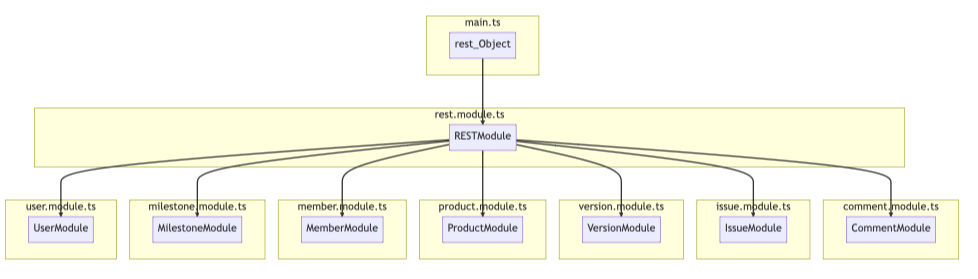
\includegraphics[width=1\textwidth]{backendmodules.png}
    \caption{Struktur der Module.tsx}
    \label{fig: backendmodules}
\end{figure}

Für jede Entität im Datenmodell ist im Verzeichnis ''packages/backend/src/modules/rest'' ist ein Ordner angelegt, welcher eine ''controller'', ''module'' und ''service'' Datei beinhaltet. In der ''module'' Datei wie zum Beispiel der product.module.ts wird definiert, welche Klassen die Aufgabe des Controllers, bzw. des Services übernehmen und welche Klassen importiert bzw. exportiert werden [siehe Abb. \ref{fig: moduleimport} auf S.~\pageref{fig: moduleimport}]. Die exportierte Klasse ''ProductModule'' wird, so wie die anderen Module der Endpunkte auch, in der ''rest.module.ts'' wieder importiert

\begin{figure}[h]
    \centering
    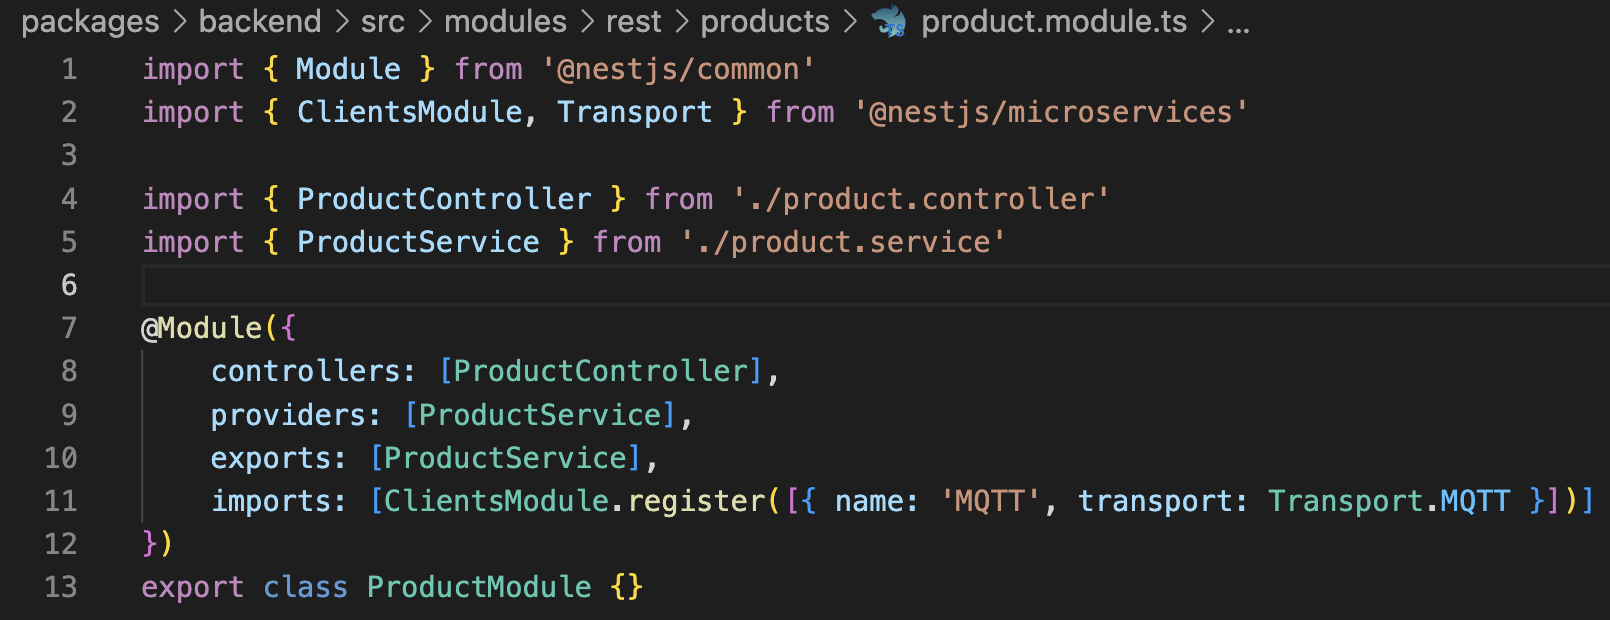
\includegraphics[width=1\textwidth]{moduleimport.png}
    \caption{Implementierung der product.module.ts}
    \label{fig: moduleimport}
\end{figure}

\section{Controller}
Der Controller hat die Aufgabe die eingehenden HTTP Requests zu empfangen und an den Service weiterzuleiten. Für die Durchführungen der ''CRUD'' Operationen werden folgende HTTP Methode verwendet:  ''Post'' um neue Daten an das Backend zu senden, ''Get'' um Daten aus dem Backend zu holen, ''Put'' um bestehende Daten zu verändern, ''Delete'' um Daten aus dem Backend zu löschen. Bevor der Controller den Service aufruft, wird noch geprüft, ob der aktuell eingeloggte User auch die Berechtigung hat die gewünschte Operation am Backend durchzuführen. Die Methoden zur Prüfung der Berechtigungen sind im der Datei ''permission.ts'' im Verzeichnis ''packages/backend/src/functions' implementiert. Diese Methoden werfen eine Exception, falls die nötigen Berechtigungen nicht vorhanden sind, und es kommt dadurch nicht dazu, dass der Controller den Service aufruft. Sind die Berechtigungen vorhanden, ruft der Controller, die im Service exportierte Funktion mit den möglichen Parametern der HTTP Nachricht auf. Dabei wird zwischen Parametern, die über den Query mitgesendet werden und Parameter, die als Body mitgesendet werden unterschieden. Als Beispiel ist als Abbildung ein ''PUT Request''. Als Query wird die ''id'' übertragen, um das gewünschte Produkt zu finden und als Body werden die neuen Daten übertragen um den Datensatz zu ändern [siehe Abb. \ref{fig: controllerput} auf S.~\pageref{fig: controllerput}]. Der Servicemethode werden die ''id'' und ''data'' mitgegeben.

\begin{figure}[h]
    \centering
    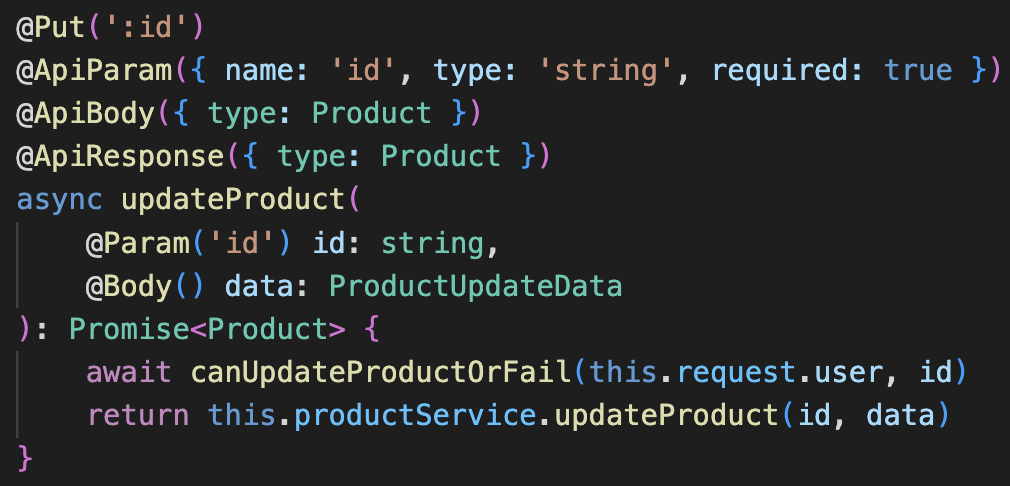
\includegraphics[width=1\textwidth]{controllerput.png}
    \caption{Implementierung von updateProduct im Controller}
    \label{fig: controllerput}
\end{figure}

\section{Service}
Im Service sind die Methoden implementiert, die die tatsächlichen Operationen auf den Daten ausführen. In der Abbildung [siehe Abb. \ref{fig: serviceput} auf S.~\pageref{fig: serviceput}]ist als Beispiel die ''updateProduct'' Methode aufgeführt. Diese Methode wird im Controller aufgerufen und es werden ihr die Parameter ''id'' und ''data'' übergeben. Als Erstes wird über die ''findOneByOrFail'' Methode zur gegebenen ''id'' ein passendes Produkt aus der Datenbank gesucht. Wird das Produkt gefunden wird es auf die Variable ''product'' geschrieben, wenn nicht, wird eine Exception geworfen. Im nächsten Schritt werden die Properties ''name'', ''description'' und ''public'' durch die Properties des übergebenen ''data'' Objektes überschrieben. Das veränderte Objekt wird mit der ''save'' Methode wieder in die Datenbank gespeichert. In der vorletzten Zeile wird eine MQTT Nachricht an das Frontend gesendet um mitzuteilen, dass der Cache nicht mehr aktuell ist, da sich ein Produkt geändert hat. Wenn das Frontend das nächste Mal nach den Produkten sucht, werden diese nicht mehr vom Cache zurückgegeben, sondern es wird ein Call ins Backend abgesetzt. Das Zusammenspiel aus Controller und Service erstreckt sich über alle Entitäten der Software und funktioniert immer nach diesem Prinzip. 

\begin{figure}[h]
    \centering
    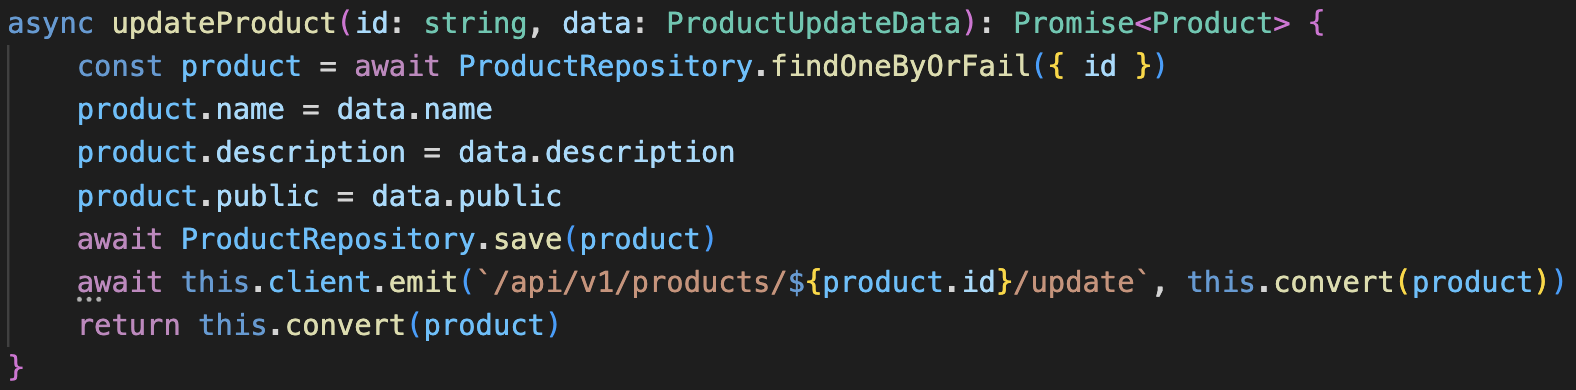
\includegraphics[width=1\textwidth]{serviceput.png}
    \caption{Implementierung von updateProduct im Service}
    \label{fig: serviceput}
\end{figure}

